\chapter{Desarrollo}


\section{En una tabla registre los porcentajes de solución salina en una columna y en la segunda columna los valores correspondientes de conductividad. Recuerde que cada valor de conductividad de esta tabla es el promedio de algunos datos de conductividad registrados durante el procedimiento. Describir este detalle.}

En la tabla \ref{tab:conductividad-mezclas} se muestra la conductividad para cada porcentaje de solución salina mezclada con agua destilada para cada caso, obteniendo diferentes valores en función del incremento del suero en la mezcla.

\begin{table}[h]
	\centering
	\begin{tabular}{|c|c|}
		\hline
		\textbf{\% Solución salina} & \textbf{Conductividad {[}uS{]}} \\ \hline
		0                           & 25.5841                         \\ \hline
		41.667                      & 1469.7841                       \\ \hline
		53.57                       & 1823.1499                       \\ \hline
		75                          & 2442.5148                       \\ \hline
		100                         & 4203.4653                       \\ \hline
	\end{tabular}
	\caption{Conductividad medida mezcla suero fisiológico + agua destilada}
	\label{tab:conductividad-mezclas}
\end{table}

Este incremento guarda correlación con el incremento de iones en le mezcla que incrementa la conductividad en cada caso, además para la obtención de la conductividad se tomo el promedio de las muestras obtenidas mediante el sensor Neulog proporcionado en el laboratorio.


\section{Qué función matemática se ajusta mejor a los puntos de \% (eje X) y de conductividad (eje Y)?}

En función a la figura \ref{fig:curva-ajuste-conductividad} la ecuación de mejor ajuste para los datos obtenidos en una ecuación lineal debido a que el conjunto de datos se ajusta con un 96.21\% en comparación a otros modelos con el polinómico (2do grado o más) o exponencial.

\begin{figure}[h]
	\centering
	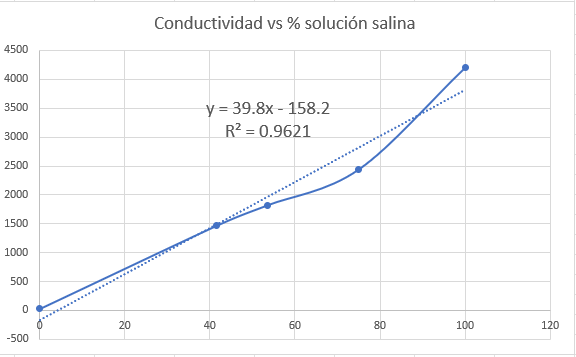
\includegraphics[width=0.7\linewidth]{media/curva-ajuste-conductividad}
	\caption{Curva de ajuste conductividad}
	\label{fig:curva-ajuste-conductividad}
\end{figure}


\section{¿Cuál es el valor de conductividad para la solución salina preparada con agua destilada y sal? Describa el procedimiento de pesaje en la balanza analítica de laboratorio y compare con la conductividad eléctrica de la solución salina pura (suero fisiológico puro). Si hubiera diferencia, explique a a qué se debería.}

Mediante el uso del sensor Neulog, datos exportados y la obtención del promedio el valor de conductividad es de 7687.3267 el cual se diferencia del valor de conductividad del suero fisiológico en 200 unidades para la misma escala $\mu S$ siendo así que para su obtención de tal valor aproximado se tuvo en cuenta la concentración de ClNa en el suero el cual corresponde 0.9g por 100ml de solución, siendo así que al contar con una muestra de 50ml de agua destilada se peso el valor aproximado de 0.45g de sal para realizar una aproximación de tal valor.

Sin embargo con este primer aproximamiento no fue posible obtener un valor cercano, por lo que se agregaron 20ml de agua destilada adicional para lograr el resultado mencionado, esto sin agregar un adicional en sal.


\section{Para la medición de conductividad del agua potable, si ésta pudiera ser descrita como una solución de cloruro de sodio (sal) en agua destilada, cuántos gramos de sal habría en cada litro de agua potable?}

El agua potable tiene un conductividad de 393.0970297 µS/cm. Para hallar la cantidad de gramos de salo por litro de agua potable es necesario analizar la conductividad para 25°C, considerando que la conductividad aumenta 2\% por °C para 25°C se tendría una conductividad de 476 µS/cm, con este valor se estime la concentración de NaCl usando la relación experimental (válida hasta 0.1 g/L) donde 0.02 g/L corresponde aproximadamente a 390 µS/cm, interpolando linealmente se tiene:

\begin{align}
	x = \frac{0.02x3900.02}{393.097}\\
	x = 0.19842 \frac{g}{L}
\end{align}

Por lo tanto, a 17.3 °C, la medición de 393.0970297 µS/cm corresponde aproximadamente a una concentración de 198 mg/L de NaCl para agua potable como una solución simple de sal.


\section{Si los líquidos en que hizo las mediciones hubieran estado a 37°C en vez de 24°C (temperatura ambiente que se puede asumir), ¿qué se esperaría de las mediciones de conductividad a esa temperatura hipotética?}


Si las mediciones de conductividad se hubieran realizado a 37°C en lugar de 24°C, se esperaría que los valores de conductividad aumentaran. Esto se debe a que la conductividad eléctrica de una solución depende de la movilidad iónica, la cual se incrementa con la temperatura. A mayor temperatura, las moléculas del disolvente (agua) presentan mayor energía cinética, lo que disminuye la viscosidad y facilita el movimiento de los iones (como Na y Cl en el suero fisiológico). En consecuencia, los iones pueden desplazarse con mayor rapidez bajo la influencia del campo eléctrico, aumentando la corriente y, por tanto, la conductividad.

En términos cuantitativos, este aumento suele ser de aproximadamente 2\% por cada grado Celsius en soluciones acuosas. Por lo tanto, al pasar de 24°C a 37°C (una diferencia de 13°C), la conductividad podría incrementarse en torno a un 26\%, manteniendo la misma concentración iónica.



% ================================================== //////////////  ================================================



\section{Según la teoría, cuál es la frecuencia de oscilación del oscilador puente de Wien en función de las resistencias y capacitancias de esa etapa del circuito y cuál fue la frecuencia que se obtuvo y que fue medida en el osciloscopio?}

\subsection{Frecuencia de oscilación teórica}

El circuito simulado en la figura \ref{fig:circuito-oscilador} corresponde a un oscilador de puente de Wien el cual se implemento con el amplificador operacional TL072CP y con el cual se genera una señal senoidal mediante una red de realimentación selectiva en frecuencia formada por resistencias y capacitores que hacen de brazos para el puente como se describe en \cite{horowitz_art_electronics}, en este tipo de oscilador la frecuencia de oscilación depende únicamente de los valores de las resistencias y capacitancias que conforman la red RC, mientras que el resto de los componentes del circuito se encargan principalmente de asegurar que la oscilación se inicie y se mantenga estable sin producir saturación excesiva del amplificador.

\begin{figure}[h]
	\centering
	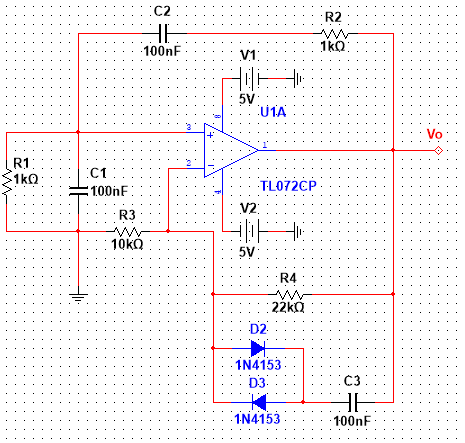
\includegraphics[width=0.5\linewidth]{media/circuito-oscilador}
	\caption{Circuio oscilador - Puente Wien}
	\label{fig:circuito-oscilador}
\end{figure}

En el circuito, la red compuesta por \(R_1\), \(R_2\), \(C_1\) y \(C_2\) se implemento como se muestra en la figura \ref{fig:amp-transimpedencia} que además del puente Wien este constituye el amplificador de transimpedancia y la etapa de rectificación para la medición de la conductividad. Por otro lado en el puente Wien cuando los valores de los componentes cumplen la condición \(R_1 = R_2 = R\) y \(C_1 = C_2 = C\), la frecuencia de oscilación del sistema puede determinarse mediante la expresión

\[
f_0 = \frac{1}{2\pi RC}
\]


\begin{figure}[h]
	\centering
	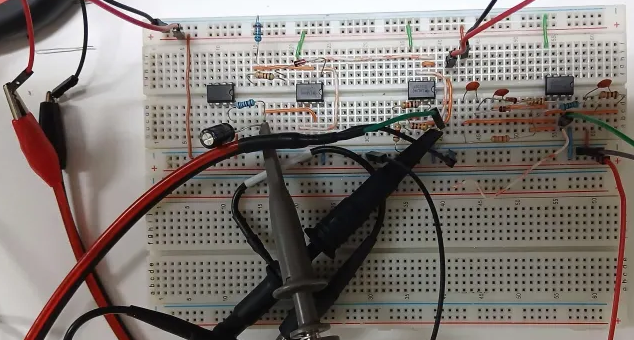
\includegraphics[width=0.6\linewidth]{media/amp-transimpedencia}
	\caption{Amplificador de transimpedancia}
	\label{fig:amp-transimpedencia}
\end{figure}

En el circuito se tienen los valores \(R = 1\,\text{k}\Omega\) y \(C = 100\,\text{nF}\). Sustituyendo estos valores en la ecuación anterior se obtiene

\[
f_0 = \frac{1}{2\pi (1000)(100 \times 10^{-9})}
\]

de lo cual se deduce que la frecuencia de oscilación es:

\[
f_0 \approx 1.56K \, \text{Hz}
\]

Por lo tanto, la frecuencia de oscilación del circuito es aproximadamente \(1.59\) kHz. A esta frecuencia la red RC introduce un desfase total de \(0^{\circ}\) y una atenuación de aproximadamente un tercio de la señal aplicada. Debido a esta atenuación, el amplificador debe proporcionar una ganancia suficiente para cumplir la condición de oscilación establecida por el criterio de Barkhausen.

La ganancia del amplificador operacional en esta configuración es la de un amplificador no inversor determinado por las resistencias \(R_3\) y \(R_4\). La expresión de la ganancia es

\[
A_v = 1 + \frac{R_4}{R_3}
\]

Sustituyendo los valores del circuito \(R_3 = 10\,\text{k}\Omega\) y \(R_4 = 22\,\text{k}\Omega\) se obtiene

\[
A_v = 1 + \frac{22\,\text{k}\Omega}{10\,\text{k}\Omega}
\]

lo cual produce

\[
A_v \approx 3.2
\]

Esta ganancia es ligeramente mayor que tres. En un oscilador de puente de Wien la ganancia ideal para mantener oscilaciones constantes es aproximadamente igual a tres, ya que la red RC atenúa la señal en un factor de \(1/3\). Al ser la ganancia inicial ligeramente mayor, se asegura que las oscilaciones puedan iniciarse a partir del ruido interno del circuito.

Además del circuito adicionalmente se puede analizar la parte de limitación con los diodos \(D_2\) y \(D_3\) que cumplen la función de control automático de amplitud. Estos diodos están conectados en antiparalelo dentro de la red de realimentación negativa. Cuando la amplitud de la señal de salida es pequeña, los diodos permanecen en estado de corte porque la tensión aplicada es menor que su tensión de conducción aproximada. En esta condición el circuito presenta la ganancia calculada previamente, lo que permite que la amplitud de la señal aumente progresivamente hasta establecer la oscilación.

\subsection{Frecuencia de oscilación Experimental}

De forma análoga en la implementación durante el desarrollo del laboratorio la frecuencia de oscilación obtenida fue de 1.5K Hz como se muestra en la figura \ref{fig:freq-oscilacion}.

\begin{figure}[h]
	\centering
	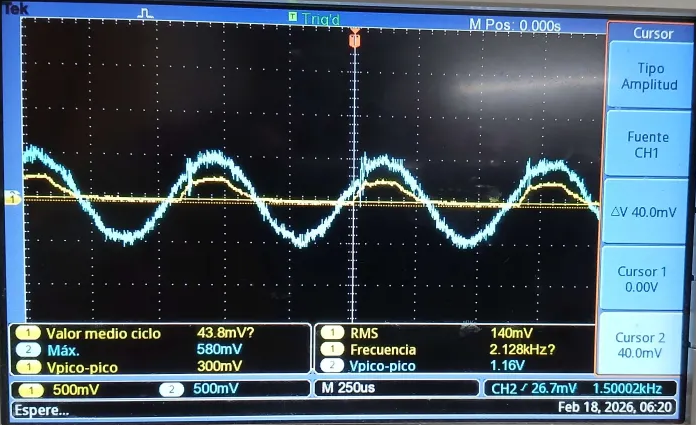
\includegraphics[width=0.5\linewidth]{media/freq-oscilacion}
	\caption{Señal senoidal generada}
	\label{fig:freq-oscilacion}
\end{figure}


\section{Explique las etapas y el funcionamiento de todo el circuito del medidor analógico de conductividad}


El circuito mostrado está compuesto por varias etapas basadas en amplificadores operacionales TL072CP y constituye un sistema de acondicionamiento analógico diseñado para procesar la señal proveniente de un oscilador senoidal, como el oscilador de puente de Wien descrito previamente y el cual uso para realizar mediciones de conductividad eléctrica, la señal senoidal generada por el oscilador se aplica a una celda de conductividad que contiene el líquido a medir. La impedancia eléctrica de la solución depende directamente de su concentración iónica, por lo que la corriente o el voltaje resultante varía de acuerdo con la conductividad del medio. El circuito mostrado procesa esa señal alterna y finalmente produce una señal continua proporcional a la conductividad del líquido.


En la figura \ref{fig:imp-amp-transimpedancia} se muestran las diferentes etapas implementadas a nivel de simulación para facilitar su comprensión.

\begin{figure}[h]
	\centering
	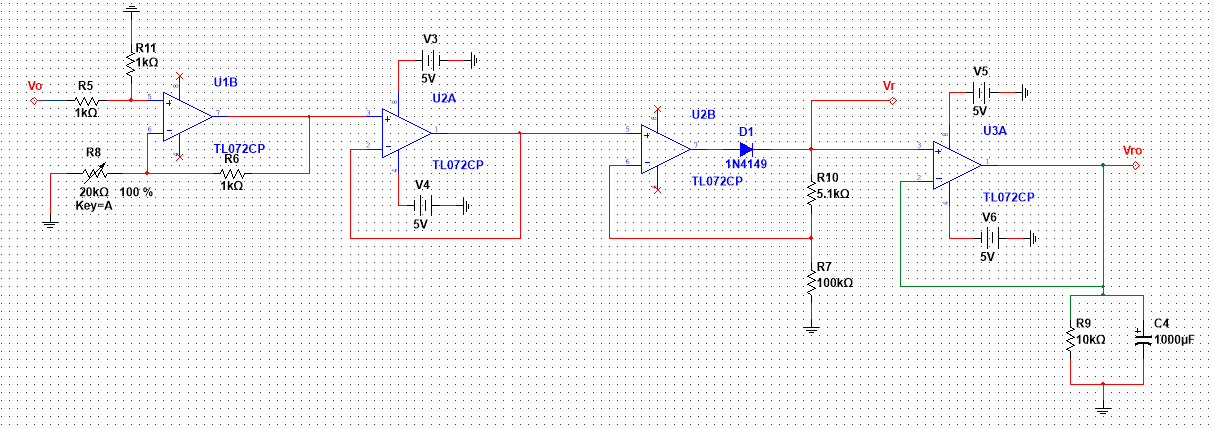
\includegraphics[width=0.8\linewidth]{media/imp-amp-transimpedancia}
	\caption{Circuito Amplificador de Transimpedancia - Medición de conductividad}
	\label{fig:imp-amp-transimpedancia}
\end{figure}

\subsection{1ra etapa - Amplificador de entrada}
La primera etapa del circuito corresponde a un amplificador de entrada la cual recibe la señal proveniente del oscilador a través de la resistencia R5 de entrada correspondiente a 1k $\Omega$, mientras que el potenciómetro en conjunto con las resistencias asociadas al mismo operacional ajustan la ganancia y establecer un punto de referencia para la señal.


\subsection{2da etapa - Seguidor de voltaje}

La segunda etapa está formada por el siguiente operacional funciona como un seguidor de voltaje o buffer obteniendo en esta configuración que la salida del amplificador se realimenta directamente a la entrada inversora, por lo que la ganancia es aproximadamente igual a uno y con la cual se logra aislar la etapa de amplificación y las siguientes etapas del circuito evitando que las impedancias de los bloques posteriores alteren la señal amplificada.

\subsection{3ra etapa - Rectificador de precisión}

La tercera etapa corresponde a un rectificador de precisión el cual a diferencia de un rectificador convencional basado únicamente en diodo permite rectificar señales de muy baja amplitud sin que la caída de voltaje del diodo afecte significativamente la señal proveniente del oscilador y modulada por la conductividad del medio se convierte en una señal unipolar. El diodo conduce durante una parte del ciclo de la señal y bloquea la otra parte, produciendo una señal rectificada cuya amplitud sigue siendo proporcional al nivel de conductividad medido.


\subsection{4ta etapa - Seguidor de voltaje y filtrado RC}

En la 4ta y última etapa está implementada un seguidor de voltaje con filtrado pasabajo en la salida conformado por una capacitancia de $1000\mu F$ y una resistencia de 10K $\Omega$ que elimina las variaciones rápidas de la señal rectificada, produciendo un valor promedio o componente continua de la señal, definiendo una DC o continua en la salida proporcional a la conductividad del liquido a analizar.

\subsection{Resumen para cada etapa}

Finalmente y como resumen, cada bloque del circuito cumple una función específica dentro del sistema de medición. La primera etapa amplifica la señal proveniente del sensor para mejorar su resolución. La segunda etapa actúa como buffer para aislar eléctricamente los bloques y evitar efectos de carga. La tercera etapa realiza la rectificación de precisión, permitiendo transformar la señal alterna en una señal unidireccional proporcional a su amplitud. Finalmente, la última etapa filtra la señal rectificada para obtener un valor promedio estable que puede ser utilizado por sistemas de adquisición de datos, microcontroladores o instrumentación digital. En conjunto, este circuito constituye un acondicionador analógico de señal para medición de conductividad, transformando una señal senoidal dependiente de la conductividad en una señal continua fácilmente interpretable por sistemas electrónicos de medición.


\section{A su grupo se le indicó un voltaje de salida determinado para un valor de conductividad eléctrica máxima a medir así como una geometría de los electrodos que se sumergirán en el liquido. cuál es el valor de resistencia equivalente de los electrodos para su conductividad}

En la figura \ref{fig:electrodos-conductividad} se muestra el electrodo con el cual se realizaron las mediciones de conductividad y cuyas puntas tienen una forma cilíndrica adecuada a la forma del cable conductor utilizado para su construcción. 

\begin{figure}[h]
	\centering
	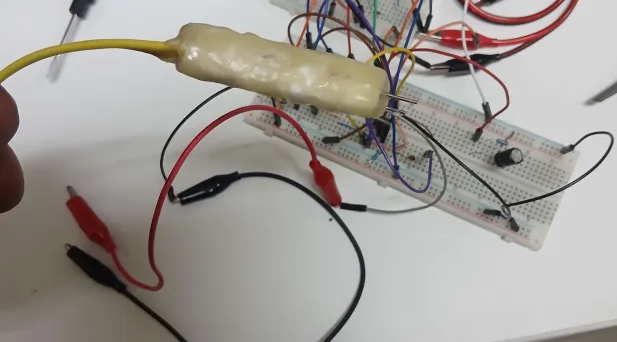
\includegraphics[width=0.7\linewidth]{media/electrodos-conductividad}
	\caption{Electrodos}
	\label{fig:electrodos-conductividad}
\end{figure}

Por otro lado el voltaje máximo medido con el sensor de conductividad elaborado corresponde a 308mV y el cual se corresponde con una resistencia equivalente a 130.0842 $\Omega$ en comparación a las mediciones realizadas con el neulog y el valor de conductividad asociado.




